\documentclass[conference]{IEEEtran}
\IEEEoverridecommandlockouts
% The preceding line is only needed to identify funding in the first footnote. If that is unneeded, please comment it out.
\usepackage{cite}
\usepackage{amsmath,amssymb,amsfonts}
% \usepackage{algorithmic}
\usepackage{graphicx}
\usepackage{textcomp}
\usepackage{xcolor}
\usepackage{algorithm}
\usepackage{subcaption}
\usepackage{algpseudocode}
\usepackage{CJKutf8}
\usepackage{mwe} % For dummy images
\def\BibTeX{{\rm B\kern-.05em{\sc i\kern-.025em b}\kern-.08em
    T\kern-.1667em\lower.7ex\hbox{E}\kern-.125emX}}
\begin{document}

\title{Using Genetic Algorithms to Explore Germinal Center Mutation Strategies}
% {\footnotesize Project for Complex Adaptive Systems }
% \thanks{Identify applicable funding agency here. If none, delete this.}
% }

\author{\IEEEauthorblockN{Connor Frost}
\IEEEauthorblockA{\textit{Computer Science} \\
\textit{University of New Mexico}\\
Albuquerque, United States \\
frostc@unm.edu}
\and
\IEEEauthorblockN{Craig Parry}
\IEEEauthorblockA{\textit{Computer Science} \\
\textit{University of New Mexico}\\
Albuquerque, United States \\
parryc@unm.edu}
\and
\IEEEauthorblockN{Michael Adams}
\IEEEauthorblockA{\textit{Computer Science} \\
\textit{University of New Mexico}\\
Albuquerque, United States \\
mikethebos@unm.edu}
}

\maketitle

\begin{abstract}

% Things to address
%   - We would like to explore cellular automata, specifically Neural Cellular Automata(NCA) and compare our results to traditional cellular automata. We have found an interesting thread on Differential Self Organizing Systems[1], which we are going to use for the basis of our exploration. Our work will include addressing the following components with respect to neural cellular automata:
% 
% 

Our project explores the recent innovations of Neural Cellular Automata's with relation to different datasets. Neural Cellular Automata (NCAs) leverage a deep learning network to both perceive and potentially react to its surrounding in a way that is similar to traditional CAs. By leveraging deep learning networks, this allows a non-discrete solution to CA rules and easier allows the NCAs to learn from well-established supervised datasets. 

This exploration with varying MNIST (Modified National Institute of Standards and Technology) datasets help us compare the results to state of the art results achieved by other models. This offers unique insights into the classification abilities of NCAs and the various problems that can be solved by this emerging technology.

\end{abstract}


\section{Introduction}

In traditional Cellular Automata (CA), there consists of a n-dimensional grid of cells where each cell consists of an on or off state. At each iteration, the grid is processed according to the ruleset and a new grid is generated. This iterative process of calculating the next iteration leads to interesting results. The most famous example of a 2D cellular automata is considered to be Conway's Game of Life, where a player creates an input and the evolutionary ruleset determines the output of the game. In neural cellular automata, the 3x3 convolution layer takes the place of a window for each grid cell. As seen in Fig 2, continuous-valued convolutions provide each cell the information about its neighborhood needed to update itself. A NCA's Convolutions provide two new abilities; They allow a cell's state to be in the range of continuous real numbers rather than discrete values, and any differentiable function can be used and will thus yield more sophisticated behavior than a regular CA. Theoretically, this has the ability to solve more complex problems. 

In terms of the cost of computation, neural networks and cellular automata can both take advantage of parallelism. However, neural networks are said to be expensive since high end graphics processing units (GPUs) are generally needed to perform training in a reasonable amount of time. This is due to the complexity involved in performing back-propagation using gradient descent during supervised learning.

In our project we adapt and extend the code developed by the self-organizing NCA series \cite{selforg}, to accomplish these classification and generative approaches to data. We also look adversarial approaches and the overall cost of computation.


% Things to address
%   - Introduce Cellular Automata and the related Neural CAs that are proposed
%   - Discuss what makes NCAs more better by using Deep Learning
%   - Fundamentals of this stuff is based on deep learning where gradients are propagated and etc. Probably a simple graph of the CNNs used.
%   - Probably a few formulas as well for consistency.

\section{Datasets}

\subsection{Overview of Fashion MNIST}

The Fashion MNIST dataset is considered a clothing and accessory dataset consisting of ten classes: T-shirt/top, Trouser, Pullover, Dress, Coat, Sandal, Shirt, Sneaker, Bag, Ankle boot. The dataset consists of 60,000 training images, and 10,000 validation images, all of which are 28x28 pixels grayscale images. This is a MNIST-like dataset (similar to the dataset presented in the base paper) and is often used as a drop-in dataset. The background of the base images are typically solid black which helps us to differentiate between what is considered the "alive" cells and the dead cells. 

\begin{figure}[htbp]
\centering{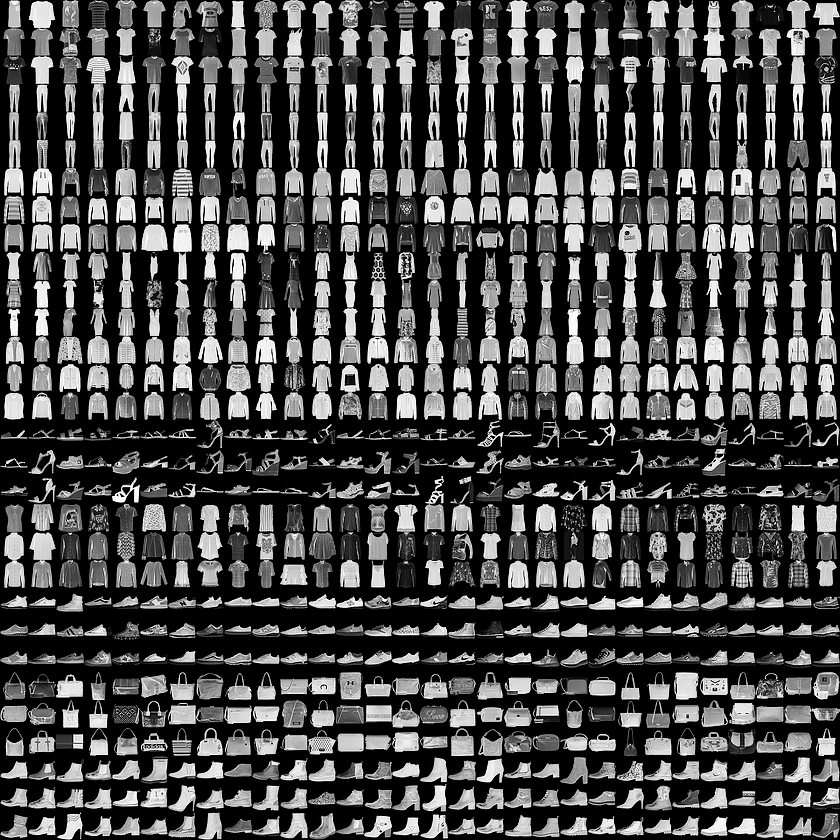
\includegraphics[scale = .4]{resources/fashion_mnist.png}}
\caption{ Visualization of a subset of images from the Fashion MNIST dataset that is trained upon, in order from top to bottom: T-shirt/top, Trouser, Pullover, Dress, Coat, Sandal, Shirt, Sneaker, Bag, Ankle boot } 
\end{figure}

The current state of the art results for the models is 96.91\% achieved by the DARTS model \cite{Darts}, and where even the most simple of dense neural networks can achieve up to 91\% \cite{tf_fmnist}. Typically, model confusion arises in the classification of items such as t-shirts, pullovers, coats, and shirts where even human-level analysis can fail.

\subsection{Overview of Kuzushiji MNIST}

The Kuzushiji MNIST (KMNIST) dataset is composed of Japanese language characters consisting of the ten main classes of Hiragana: \begin{CJK}{UTF8}{min} お, き, す, つ, な, は, ま, や, れ, を \end{CJK}. \cite{kmnist} KMNIST is constructed similarly to Fashion MNIST with 28x28 grayscale images composing a training set of 60,000 examples, and a test set of 10,000 examples. It can be used as a drop-in replacement for MNIST and its color space allows for easy adaptation into NCA models.

\begin{figure}[htbp]
\centering{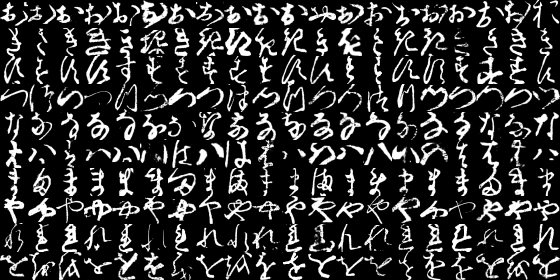
\includegraphics[scale = .4]{kmnist/adv_demo/composite.png}}
\caption{ Visualization of a subset of images from the KMNIST dataset that is trained upon. Each row represents a class of Hiragana; modern calligraphy is used on the left and ages as read from left to right.} 
\end{figure}

State of the art models \cite{kmnistsota} achieve 99.76\% with shake-shake regularization in order to minimize overfitting. In contrast to MNIST, Hiragana characters are mostly non-contiguous, meaning that they tend to feature islands of strokes separated by white space. This will prove significant to our NCA implementation since each input image is segmented into alive and dead cells.

\section{Methods}

\subsection{Data Preprocessing}

There is fundamentally an innate segmentation task of partitioning "alive" cells (where the NCAs would be calculated) and the dead cells. In images, the alive cells would be defined by the pixels of the object subject to classification excluding the background. We do much of this data preprocessing by filtering out the background this is typically the darkest cells in the image, and manually calculate the alive cell mask.

Although there are specifically computer vision datasets for image segmentation, for simplicity we use both the Fashion MNIST and the KMNIST datasets. These are well known formats and we are able to differentiate the background from the foreground via filtering out the dark pixels with great accuracy. Unfortunately, it does seem that sometimes the clothing items such as the ones found in the Fashion MNIST dataset occasionally have dark pixels within the center. We suspect that this is due to the inclusion of graphic designs such as t-shirts where the design once converted to grayscale becomes dark enough to be filtered out with the background. Fortunately, we are able to still show model viability with regards to the dataset even with the included noise in the training data. 
 
The input images for the neural cellular automata are normalized by rescaling the gray-scale pixel vaues between 0 and 1. By introducing a threshold of 0.1 to differentiate the background (consisting of dead-cells) from the foreground (which are considered light-cells). 

\begin{figure}[htbp]
\centering{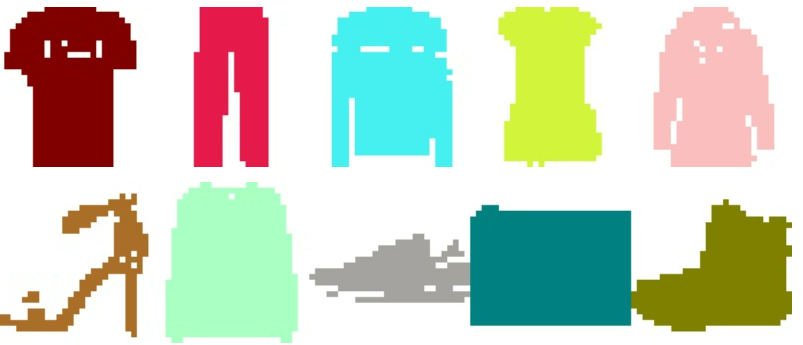
\includegraphics[scale = .4]{resources/sample_vis_fmnist.png}}
\caption{Sample training set visualization of each clothing item with its corresponding colored-classification in the Fashion MNIST dataset }
\end{figure}

\section{Models}

The models typically rely on two different model configurations that are used in conjunction: the perception model, and the decision model. The goal of the perception model is to emulate the perception of surrounding neural cellular automata. The goal of the decision model is to decide the update step and apply a stochastic update.

The following loss functions are considered to make back-propagation feasible for "alive" cells:

\begin{itemize}
    \item L2 Norm
    \item Cross-Entropy
    \item Sparse Categorical Cross-Entropy (after a softmax activation function)
\end{itemize}

\subsection{Generative Model}

Since the goal of the model is to regenerate an image that the neural cellular automata was trained upon, the output of the decision model must be the update state for that pixel. Since the process of regenerating the image from a single "alive" cell, the number of alive and dead cells must be dynamic in nature for the complex interactions to grow. To accomodate this, at the end of each update step, new cells may be chosen around existing alive cells to allow for the growth of the generative model at the end of each update step.

\begin{itemize}
    \item Input Layer: 28x28 color image.
    \item Perception Model - Layer 1: 2D Convolutional Neural Network with 3x3 kernel sobel operator (used for edge-detection) where padding is conserved.
    \item Decision Model - Layer 1: 2D Convolutional Neural Network, fully connected with ReLU activation function
    \item Decision Model - Layer 2: 2D Convolutional Neural Network with 16 outputs for update on each pixel.
\end{itemize}


\subsection{Classification Model}

The classification model is of similar form to the generative model with a perception and decision model. However, the decision model's goal becomes to output the correct classification of the pixel of the image and thus requires an activation function capable of producing a probability distribution function indicating the likelihood of each respective class. The perception model with the classification uses a trainable 2D convolutional neural network instead of the sobel operator in an attempt to better learn the features of the object.

\begin{itemize}
    \item Input Layer: 28x28 grayscale image.
    \item Perception Model - Layer 1: Convolutional Neural Network with 3x3 kernel operator where padding is conserved
    \item Decision Model - Layer 1: Flatten output of perception model into 1D array
    \item Decision Model - Layer 2: 128 nodes, fully connected with ReLU activation function
    \item Decision Model - Layer 3: 10 nodes with classification-able activation function 
\end{itemize}

The authors in \cite{self-classify} change the target image and class every 200 steps. This is done to ensure that each cell in the NCA is able to continuously classify rather than get stuck in a dormant state where the output classification never changes. In each of our training plots throughout the Results sections, this is visible as a discontinuity at step 200.

\subsection{Adversarial Model} 

The adversarial begins with a pre-trained classification model and selects neural cellular automata to hijack. This is accomplished by modifying the training data to be intentionally corrupted and thus training the neural cellular automata using the "bad" data. Then, the original classification model has neural cellular automata repalaced with the adversarially trained neural cellular automata to maximize error. 

\section{Fashion MNIST Results}

\subsection{Fashion MNIST Classification Results}

After training the classification model on the Fashion MNIST dataset, that has been preprocessed and normalized, for 100,000 epochs. The general accuracy of the model is calculated to be the following:

\begin{equation}
    \frac{Total\_Correct\_CAs} {Total\_CAs}
\end{equation}

The maximum final accuracy determined from the test dataset is calculated to be 80.81\%.

\begin{figure}[htbp]
\centering{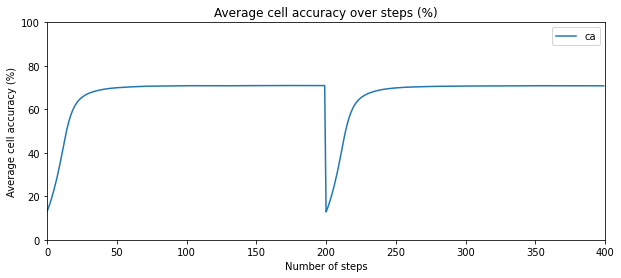
\includegraphics[scale = .4]{resources/test_accuracy.png}}
\caption{Three dimensional box plot of the mean hamming distance between the adjusted probabilities on an }
\end{figure}



Unfortunately, this metric is not the most informative metric as it doesn't account for agreement between cells. A secondary metric can be applied here as the agreement between cells. This can be computed as the ratio of samples where all the cells output the same label to the total number of samples.

\begin{figure}[htbp]
\centering{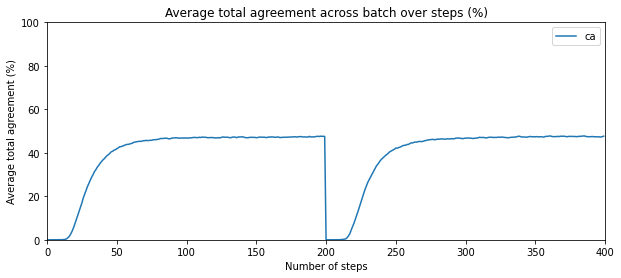
\includegraphics[scale = .4]{resources/test_agreement.png}}
\caption{ Total agreement amongst pixels with respect to the classification that is being outputted for the Fashion MNIST dataset.}
\end{figure}

By introducing this secondary metric, this attempts to help account for convergence of classifications amongst local regions with respect to each image. This metric becomes especially important with data that is not spatially connected. Due to the noise introduced in the pre-processing for the fashion MNIST dataset, there are occasionally "islands" of pixels that arrive to different classifications sometimes irrelevant to object of interest's classification.

\begin{figure}
    \centering
    \begin{minipage}{0.24\textwidth}
        \centering
        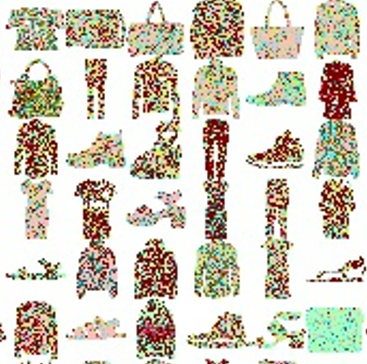
\includegraphics[width=0.9\textwidth]{resources/ep100_class.png} % first figure itself
        % \caption{first figure}
    \end{minipage}\hfill
    \begin{minipage}{0.24\textwidth}
        \centering
        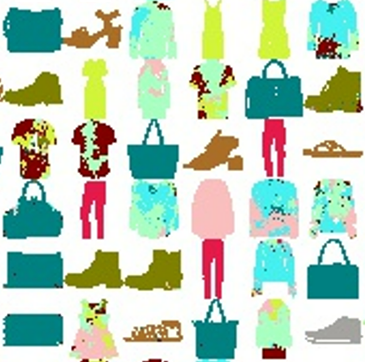
\includegraphics[width=0.9\textwidth]{resources/ep100000_class.png} % second figure itself
        % \caption{second figure}
    \end{minipage}
    \caption{Left: Visualization of training progress at epoch 100. Right: Visualization of training progress at epoch 100,000}
    \label{fig:fig}
\end{figure}


Given the visualizations provided in fig. 5, the models become more proficient at classification as training progresses. 

\subsection{Fashion MNIST Generative Results}

Using the generative model, we can train the neural cellular automata to regenerate an image that it was trained upon. This relies on an iterative approach to defining the alive and dead cells with each iteration. Upon each iteration, the cellular automata have been trained to generate the next iteration. However, the model is still limited by the designated alive cells. 

Because the alive cells in the generative results are dynamic. The selection of "new" cells to switch on must be performed after each iteration. The best way of going about this is to switch on cells surrounding other alive cells given a threshold. This is done at the end of each iteration to allow the model to grow relative to the activity of the model. There seems to be a trade-off by increasing the number of newly switched on cells increase the instability of the results. The slow and steady approach of the model leads the results to strictly converge to the image that it was trained upon.  

\begin{table}[ht]
\begin{tabular}{cc}
\begin{subfigure}{0.23\textwidth}\centering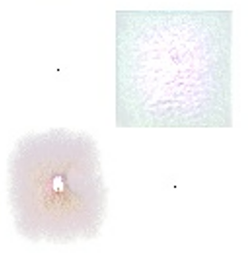
\includegraphics[width=1\columnwidth]{resources/gen_fmnist/ex100_adv.png}\caption{After 100 epochs}\label{fig:taba}\end{subfigure}&
\begin{subfigure}{0.23\textwidth}\centering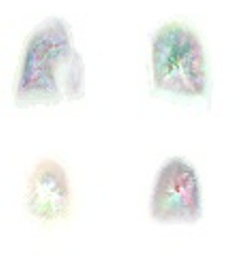
\includegraphics[width=1\columnwidth]{resources/gen_fmnist/ex500_adv.png}\caption{After 500 epochs}\label{fig:tabb}\end{subfigure}\\
\newline
\begin{subfigure}{0.23\textwidth}\centering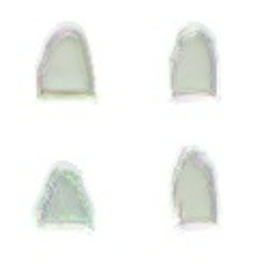
\includegraphics[width=1\columnwidth]{resources/gen_fmnist/ex1000_adv.png}\caption{After 1000 epochs}\label{fig:tabc}\end{subfigure}&
\begin{subfigure}{0.23\textwidth}\centering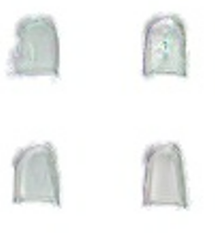
\includegraphics[width=1\columnwidth]{resources/gen_fmnist/ex2000_adv.png}\caption{After 2000 epochs}\label{fig:taba2}\end{subfigure}\\
\newline
\begin{subfigure}{0.23\textwidth}\centering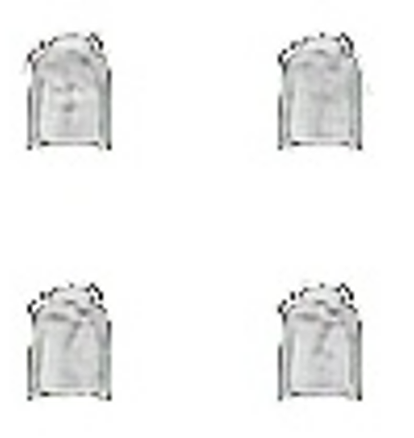
\includegraphics[width=1\columnwidth]{resources/gen_fmnist/ex5000_adv.png}\caption{After 5000 epochs}\label{fig:tabc}\end{subfigure}&
\begin{subfigure}{0.23\textwidth}\centering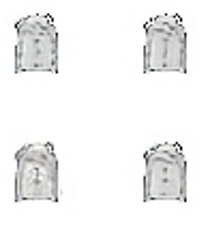
\includegraphics[width=1\columnwidth]{resources/gen_fmnist/ex8000_adv.png}\caption{After 8000 epochs}\label{fig:taba2}\end{subfigure}\\
\end{tabular}
\caption{Training progress over time in the generation of the images}
% \label{tab:mytable}
\end{table}

From the information and the generated progress visualizations, the model seems to be able to recreate the original image in many different manners, but in the end after 8000 epochs, the neural cellular automata seem to be successful in the recreation. 


\begin{figure}[htbp]
\centering{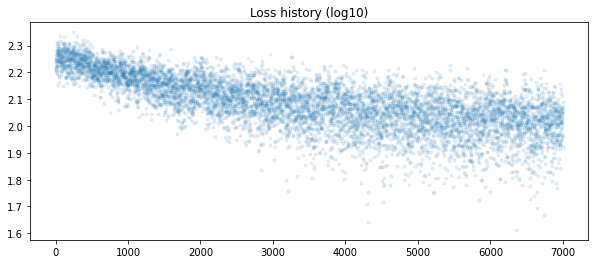
\includegraphics[scale = .4]{resources/test_losspng.png}}
\caption{Three dimensional box plot of the mean hamming distance between the adjusted probabilities on an }
\end{figure}

\subsection{Introducing Adversarial Training}

By training an adversarial classifier model and selecting the most impactful pixels, the robustness of the model can be tested by utilizing these adversarially trained neural cellular automata with the rest of the originally trained classification model. 

This is done in the following manner:
\begin{enumerate}
    \item Train a classification model normally as described in earlier sections
    \item Train an adversarial model with a distorted version of the dataset
    \item Swap out 1\% of pixels of the training model with the adversarial model
    \item Test the results.
\end{enumerate}


The training results of this model is demonstrated below and demonstrate the impactfullness of the success that the adversarial models have.

\begin{figure}[htbp]
\centering{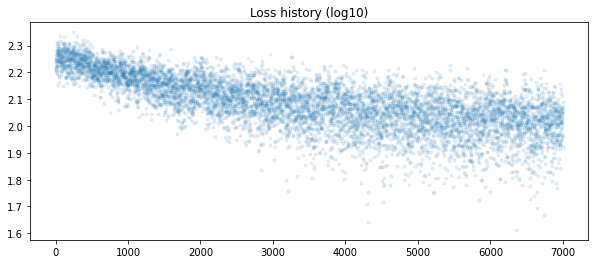
\includegraphics[scale = .4]{resources/test_losspng.png}}
\caption{Three dimensional box plot of the mean hamming distance between the adjusted probabilities on an }
\end{figure}

This is in the case of a naively

\section{Kuzushiji-MNIST Results}

\subsection{Kuzushiji-MNIST Classification Results}

The self classification model used on Fashion MNIST was also used to self-classify Japanese Hiragana character groups. Average accuracy among every pixel CA is used here to measure overall accuracy. 

\begin{figure}[htbp]
\centering{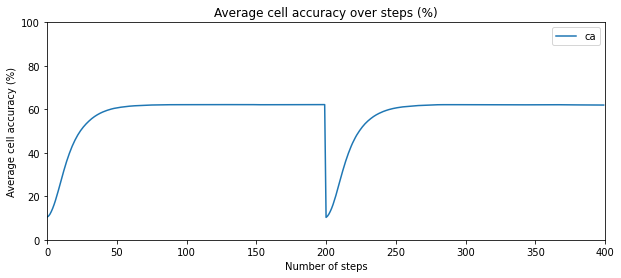
\includegraphics[scale = .4]{kmnist/avgacc.png}}
\caption{Average accuracy among CA cells for Kuzushiji-MNIST dataset.}
\label{kmnistavg}
\end{figure}

As seen in Figure \ref{kmnistavg}, the model achieves 61.97\% accuracy. However, as explained before for Fashion MNIST, agreement is a more important metric.

\begin{figure}[htbp]
\centering{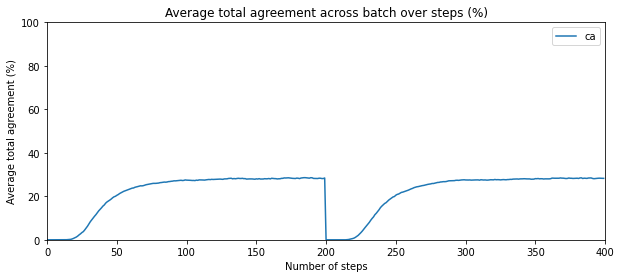
\includegraphics[scale = .4]{kmnist/agreement.png}}
\caption{ Total agreement amongst pixels with respect to the classification that is being outputted for the Kuzushiji-MNIST dataset.}
\label{kmnistagree}
\end{figure}

\begin{figure}
    \centering
    \begin{minipage}{0.24\textwidth}
        \centering
        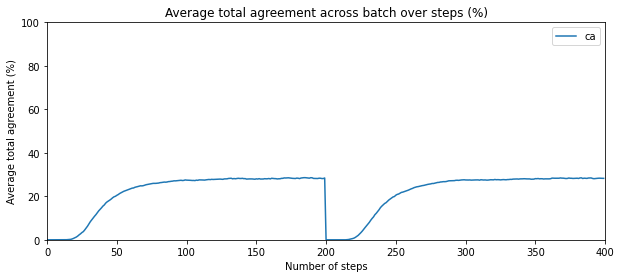
\includegraphics[width=0.9\textwidth]{kmnist/agreement.png} % first figure itself
        \caption{Total agreement amongst pixels with respect to the classification that is being outputted for the Kuzushiji-MNIST dataset.}
        \label{kmnistagree}
    \end{minipage}\hfill
    \begin{minipage}{0.24\textwidth}
        \centering
        
\includegraphics[width=0.9\textwidth]{resources/islandexamplekmnist.png} % second figure itself
        \caption{An example hiragana character that has three islands of pixels.}
        \label{kmnistislands}
    \end{minipage}
\end{figure}

Agreement is especially important with regards to Japanese Hiragana characters. Since a segmentation mask is used to prevent communication between islands of active cells, isolated calligraphic strokes present within some characters cannot communicate to converge on a consensus. Isolated strokes are common within Japanese calligraphy, so the final agreement of 28.26\% seen in Figure \ref{kmnistagree} is not surprising. 

Tu further verify the proficiency of self-classification on the KMNIST dataset, confusion matrices were used. Figure \ref{kmnistconfusion} shows the confusion matrix for a 100,000 step training run.

\begin{figure}[htbp]
\centering{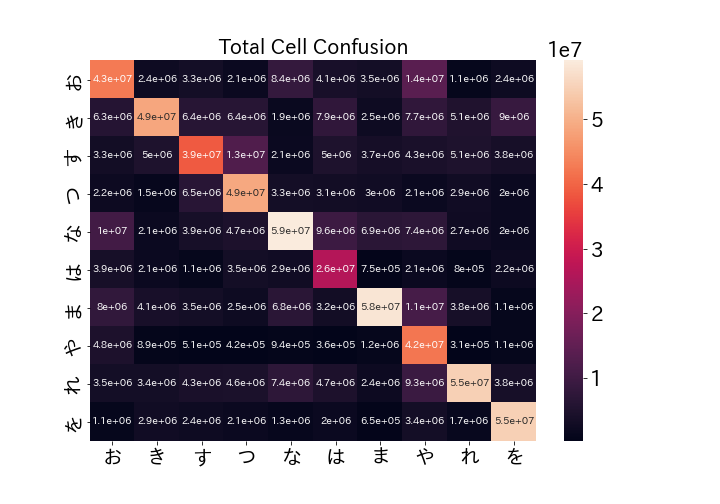
\includegraphics[scale = .4]{resources/kmnisttotalconfusion.png}}
\caption{ Final training confusion matrix for each sample in the KMNIST test data set. Each row in a confusion matrix corresponds to the samples in an actual class while each column corresponds to the samples in a predicted class.}
\label{kmnistconfusion}
\end{figure}

It can be seen that the model does fairly well at prediction once trained. Rows 2 and 5 (\begin{CJK}{UTF8}{min}き, な\end{CJK}, respectively) feature the most confusion as they have relatively high numbers of incorrect classifications in up to 4 other Hiragana character classes.  The characters corresponding to rows 2 and 5 have a diverse number of strokes taken in all directions (vertical:  up/down, horizontal:  left/right), which could be a possible cause for the confusion exhibited, especially since some of the incorrect classifications are of images that have islands of cells like those seen in Figure \ref{kmnistislands}.

\section{Discussion}

This model still achieves decent results but has an element of visualization native to the model itself. While it may not be close to the state of the art results, it may be more ideal for those who are interested in models with an explainability / visualization capability over what you would typically see in black-box neural networks. 

In addition, increasing the convolution size from 3x3 to 5x5 is completely possible to obtain better results as it increases the number of trainable parameters and also increases the scope for which results can be inferred upon. Unfortunately, this does lead to higher computation costs.

Currently, the generative model achieves the dynamic switching of cell states by turning on neighbors that go above a certain level of activity. This can be changed to become more dynamic such as moderating the total amount of new neighbors (by drastically reducing or increasing the limits), and by developing new dynamic rules for the switching. Currently, the model grows on pace with the addition of new cells and regeneration of the original image, however, increasing the instability may allow for the model to regenerate with some added variances.

\section{Conclusion}


\begin{thebibliography}{00}

\bibitem{selforg} Mordvintsev, Alexander, et al. “Growing Neural Cellular Automata.” Distill, 27 Aug. 2020, https://distill.pub/2020/growing-ca/. 

\bibitem{self-classify} Randazzo, et al., "Self-classifying MNIST Digits", Distill, 2020.

\bibitem{adversarial} Randazzo, et al., "Adversarial Reprogramming of Neural Cellular Automata", Distill, 2021.

\bibitem{Darts} M. S. Tanveer, M. U. K. Khan, και C.-M. Kyung, ‘Fine-Tuning DARTS for Image Classification’, CoRR, τ. abs/2006.09042, 2020.

\bibitem{tf_fmnist} TensorFlow, TensorFlow Docs, (2020), GitHub repository, https://github.com/tensorflow/docs

\bibitem{fmnist} H. Xiao, K. Rasul, και R. Vollgraf, ‘Fashion-MNIST: a Novel Image Dataset for Benchmarking Machine Learning Algorithms’, CoRR, τ. abs/1708.07747, 2017.

\bibitem{kmnist} Clanuwat, Tarin, et al. “Deep Learning for Classical Japanese Literature.” ArXiv.org, 3 Dec. 2018, https://arxiv.org/abs/1812.01718. 

\bibitem{kmnistsota}  Hysts. “Pytorch Implementation of Image Classification Models for CIFAR-10/CIFAR-100/Mnist/Fashionmnist/Kmnist” GitHub, github.com/hysts/pytorch\_image\_classification

\end{thebibliography}

\section*{Contribution Statements}

\subsection{Connor}

\begin{itemize}
    \item Worked on getting the classification up and running for Fashion MNIST
    \item Worked on getting the Adversarial training based on previous model runs
    \item Presented the work done on the project thus far on May 3rd, 2022.
    \item Worked on Fashion MNIST slides and data preparation slides.
    \item Wrote the model overviews section
    \item Helped write the introduction, abstract, and fashion MNIST results
\end{itemize}

\subsection{Craig} 

\begin{itemize}
    \item Worked on getting generative abilities with respect to the Fashion MNIST dataset
    \item Primary writer for the proposal
    \item Assisted with work of the adversarial training of Fashion MNIST
    \item Helped write data preparation section for the final paper. Contributed to the data preparation slides for the presentation.
    \item Wrote the Overview of Fashion MNIST section for the final paper
    \item Helped write the introduction, abstract, discussion, and fashion MNIST results.
\end{itemize}

\subsection{Michael} 


\end{document}


